\documentclass[aspectratio=43]{beamer}

\usetheme[progressbar=frametitle]{metropolis}
\usepackage{appendixnumberbeamer}


\usepackage{amsmath}
\usepackage{mathtools}
\usepackage{xcolor}

\usepackage{transparent}
\usepackage{pdfpages}

\usepackage{hyperref}
\hypersetup{
    colorlinks=true,
    linkcolor=black,
    filecolor=magenta,      
    urlcolor=cyan,
}

\usepackage{array}
\usepackage{booktabs}

\usepackage{multicol}
\usepackage{vwcol}
\usepackage{wrapfig}
\usepackage[export]{adjustbox}

\usepackage{graphicx}


  % declare the path(s) where your graphic files are
\graphicspath{{media/}}
  % and their extensions so you won't have to specify these with
  % every instance of \includegraphics
\DeclareGraphicsExtensions{.pdf,.jpeg,.png}

\usepackage[utf8]{inputenc}

\usepackage[font=small,labelfont=bf]{caption}

\usepackage{helvet}
\renewcommand{\familydefault}{\sfdefault}

\DeclareCaptionFont{tiny}{\tiny}

\DeclareMathOperator*{\argmax}{argmax}
\DeclareMathOperator*{\argmin}{argmin}

%\setbeamercolor{background canvas}{bg=white}

\usebackgroundtemplate%
{%
    
\includegraphics[width=\paperwidth,height=\paperheight]{lmu_background}%
}
\newcommand\pro{\item[$+$]}
\newcommand\con{\item[$-$]}

\newcommand{\themename}{\textbf{\textsc{metropolis}}\xspace}

\newcommand{\backupbegin}{
   \newcounter{finalframe}
   \setcounter{finalframe}{\value{framenumber}}
}
\newcommand{\backupend}{
   \setcounter{framenumber}{\value{finalframe}}
}

\title{Missing Data Imputation}
\date{11.12.2019}
\author{Alexander Hanf, Arber Qoku}

\begin{document}
%
\maketitle

\begin{frame}{Agenda}
\tableofcontents
\end{frame}

\section{Statistical background}

\begin{frame}{Missing data}
\begin{itemize}
\item Very common in practical problems
\item Data can be missing for many reasons
\begin{itemize}
\item Survey participant is unreachable or refuses to answer
\item Question does not apply to patient (sex-specific)
\item Subset of sensors not working for a period of time
\end{itemize}
\item Complicates statistical analysis (bias, statistical power, ...)
\item Many machine learning models can not handle missing data.
\end{itemize}
\end{frame}

\begin{frame}{Types of missing data}
\begin{itemize}
\item Missing completely at random (MCAR): the pattern of missing values is independent of all other covariates (both observed and unobserved)
\item Missing at random (MAR): the pattern of missing values depends only on observed covariates
\item Missing not at random (MNAR): the pattern of missing values also depends on unobserved covariates
\end{itemize}
\end{frame}

\begin{frame}{Idea of Imputation}
\begin{itemize}
\item Use statistical techniques to fill in the missing values
\item Make the most of the data we have
\item Caution is required! We can bias our analysis or create nonsensical data
\end{itemize}
\end{frame}


\section{Imputation Methods}

\begin{frame}{Complete case analysis}
\begin{itemize}
\item Row-wise or column-wise deletion
\end{itemize}
\begin{itemize}
\pro Very simple
\pro Valid inferences when MCAR
\end{itemize}
\begin{itemize}
\con Biased results on MAR or MNAR
\con Too few datapoints (if any) left!\\
If only $5\%$ missing independently on a dataset with 20 columns, we end up with $0.95^{20} \approx 35\%$ of the original data\\
\end{itemize}
\textcolor{red}{Big problem in predictive modelling!}
\end{frame}

\begin{frame}{Imputation of constant values}
\begin{itemize}
\item Substitute mean, median, mode, constant value
\end{itemize}
\begin{itemize}
\pro Simple
\pro Retains all observed values
\pro Can preserve statistical quantities
\end{itemize}
\begin{itemize}
\con Underestimates standard errors
\con May impute unrealistic values
\end{itemize}
\end{frame}

\begin{frame}{Hot-Deck Imputation}
\begin{itemize}
	\item General idea: reuse values from other observations
	\item Assumption: identically distributed data points
	\item "Donor" observations can be chosen in multiple ways
	\begin{itemize}
		\item Naively: imputing value from randomly chosen observation
		\item Distance-based methods
		\item Predictive mean matching (Regression \& Distance)
	\end{itemize}
\end{itemize}
$$X = \underbrace{\begin{pmatrix}
	x_{11} 	& x_{12} 	& x_{13} \\
	x_{21} 	& x_{22} 	& x_{23} \\
	- 		& x_{32} 	& x_{33} \\
	\end{pmatrix}}_\text{original design matrix}
\rightarrow
\underbrace{
	\begin{pmatrix}
	x_{12} 	& x_{13} \\
	x_{22} 	& x_{23} \\
	\end{pmatrix}
}_\text{design matrix},
\underbrace{\begin{pmatrix}
	x_{11} \\
	x_{21} \\
	\end{pmatrix}}_\text{response}
\rightarrow
\underbrace{
	\begin{pmatrix}
	\textcolor{blue}{\hat{x}_{11}}		& x_{12} 	& x_{13} \\
	\textcolor{blue}{\hat{x}_{21}} 		& x_{22} 		& x_{23} \\
	\textcolor{blue}{\hat{x}_{31}} & x_{32} 	& x_{33} \\
	\end{pmatrix}}_\text{compute distances}
$$

\begin{itemize}
	\pro Easy to implement and computationally efficient
\end{itemize}
\begin{itemize}
	\con Donor values might get reused often
	\con Underestimates standard errors
\end{itemize}
\end{frame}

\begin{frame}{Multiple Imputation}
\begin{itemize}
\item Use given data to quantify uncertainty of imputations
\end{itemize}
\phantom{This text will be invisible} 
\centering

\includegraphics[width=0.9\paperwidth]{MI}
\end{frame}

\begin{frame}{Specification Overhead}
\begin{itemize}
%\item Missingness pattern: MCAR, MAR, MNAR
\item Imputation model: linear regression, random forest, ...
\item Predictor vs response variables: leave-one-out, interactions, auxiliary, ...
\item Order of variable imputation: random, least/most missing first, ...
\item Initial imputations, number of iterations (convergence condition)
\item Number of multiply imputed datasets (cycles)
\end{itemize}
\phantom{This text will be invisible invisible invisible invisible invisible invisible} 
\onslide<2> $\Rightarrow$ Multiple Imputation by Chained Equations (MICE)
\end{frame}

\begin{frame}{Multiple Imputation by Chained Equations (MICE)}
$$X = \underbrace{\begin{pmatrix}
x_{11} 	& - 		& x_{13} \\
x_{21} 	& x_{22} 	& - \\
- 		& x_{32} 	& - \\
x_{41} 	& x_{42} 	& x_{43} \\
\end{pmatrix}}_\text{original design matrix}
\rightarrow
\underbrace{\begin{pmatrix}
x_{11} 		& \textcolor{red}{\bar{x}_{.2}} 	& x_{13} \\
x_{21} 		& x_{22} 		& \textcolor{red}{\bar{x}_{.3}} \\
\textcolor{red}{\bar{x}_{.1}} & x_{32} 	& \textcolor{red}{\bar{x}_{.3}} \\
x_{41} 		& x_{42} 	& x_{43} \\
\end{pmatrix}}_\text{initial imputation}
\rightarrow
\underbrace{\begin{pmatrix}
\textcolor{red}{\bar{x}_{.2}} 	& x_{13} \\
x_{22} 		& \textcolor{red}{\bar{x}_{.3}} \\
x_{42} 	& x_{43} \\
\end{pmatrix}}_\text{design matrix},
\underbrace{\begin{pmatrix}
x_{11} \\
x_{21} \\
x_{41} \\
\end{pmatrix}}_\text{response}$$

$$
\rightarrow
\begin{pmatrix}
x_{11} 		& \textcolor{red}{\bar{x}_{.2}} 	& x_{13} \\
x_{21} 		& x_{22} 		& \textcolor{red}{\bar{x}_{.3}} \\
\textcolor{blue}{\hat{x}_{31}} & x_{32} 	& \textcolor{red}{\bar{x}_{.3}} \\
x_{41} 		& x_{42} 	& x_{43} \\
\end{pmatrix}
\rightarrow
\begin{pmatrix}
x_{21} 		& \textcolor{red}{\bar{x}_{.3}} \\
\textcolor{blue}{\hat{x}_{31}} & \textcolor{red}{\bar{x}_{.3}} \\
x_{41} 		& x_{43} \\
\end{pmatrix},
\begin{pmatrix}
x_{22} \\
x_{32} \\
x_{42} \\
\end{pmatrix}
\rightarrow
\cdots
\underbrace{\begin{pmatrix}
x_{11} 		& \textcolor{blue}{\hat{x}_{12}} 	& x_{13} \\
x_{21} 		& x_{22} 		& \textcolor{blue}{\hat{x}_{23}} \\
\textcolor{blue}{\hat{x}_{31}} & x_{32} 	& \textcolor{blue}{\hat{x}_{33}} \\
x_{41} 		& x_{42} 	& x_{43} \\
\end{pmatrix}}_{X_i^{*}}
$$
%\onslide<2>\textcolor{red}{Do we actually need multiple datasets in predictive modelling?}
\end{frame}

\begin{frame}{Deep Learning for Imputation}
\begin{itemize}
	\item Recent advances in deep learning improved model performance on a wide variety of NLP tasks
	\item This can be used to impute textual features or other categorical features
	\item Example: searching for "yellow dress" on Amazon - textual description might exist, but "colour" is missing in database
\end{itemize}
\end{frame}

\begin{frame}{Amazon DataWig}
\small scalable, high-precision, language-agnostic, end-to-end pipeline

\centering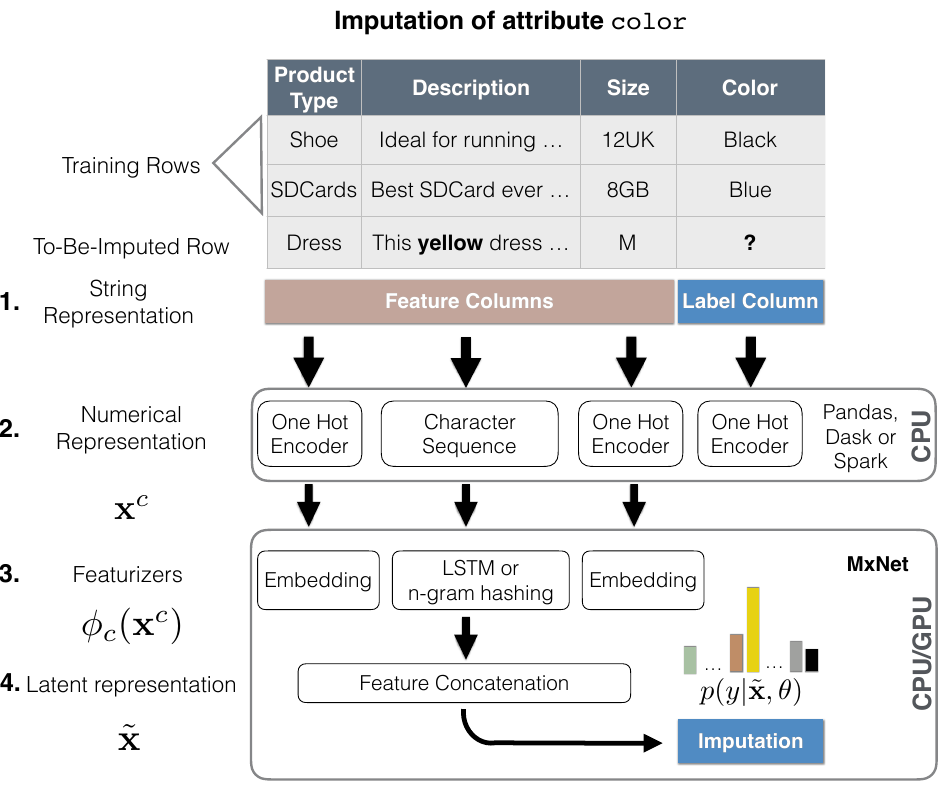
\includegraphics[width=0.7\paperwidth]{datawig}
\end{frame}

\section{Tools and libraries for dealing with missing data}

\begin{frame}{Useful libraries}
Exploratory data analysis
\begin{itemize}
\item General purpose: \href{https://github.com/pandas-profiling/pandas-profiling}{pandas-profiling}
\item Specific to missing data: \href{https://github.com/ResidentMario/missingno}{missingno}
\end{itemize}
Imputation
\begin{itemize}
\item General purpose ($\sim$\href{https://cran.r-project.org/web/packages/mice/mice.pdf}{\texttt{ mice}} in R): \href{https://scikit-learn.org/stable/modules/impute.html}{scikit-learn}
\item Hot-deck with KNNs: \href{https://github.com/iskandr/fancyimpute}{fancyimpute}
\item Random Forest ($\sim$\href{https://cran.r-project.org/web/packages/missForest/missForest.pdf}{\texttt{ missForest}} in R): \href{https://github.com/epsilon-machine/missingpy}{missingpy}
\item Imputation of Time Series Data (WIP): \href{https://github.com/eltonlaw/impyute}{impyute}
\end{itemize}
\end{frame}

\section{Live Demo}

\appendix
\begin{frame}{References}
\scriptsize
\begin{itemize}
	\item Biessmann, Felix, et al. "Deep Learning for Missing Value Imputation in Tables with Non-Numerical Data." Proceedings of the 27th ACM International Conference on Information and Knowledge Management. ACM, 2018.
	\item Buuren, S. van, and Karin Groothuis-Oudshoorn. "mice: Multivariate imputation by chained equations in R." Journal of statistical software (2010): 1-68.
	\item Wulff, Jesper N., and Linda Ejlskov. "Multiple Imputation by Chained Equations in Praxis: Guidelines and Review." Electronic Journal of Business Research Methods 15.1 (2017).
	\item Joenssen, Dieter William Hermann. Hot-Deck-Verfahren zur Imputation fehlender Daten: Auswirkungen des Donor-Limits. Diss. 2015.
\end{itemize}
\end{frame}
\end{document}
